\documentclass[a4paper, 11pt]{article}

\usepackage[utf8]{inputenc}

\usepackage[lmargin=1.5cm,tmargin=2cm,rmargin=1.3cm,bmargin=2cm]{geometry}
\usepackage[onehalfspacing]{setspace}
\usepackage[T1]{fontenc}
\usepackage[brazil]{babel}
\usepackage{float}
\usepackage{polynom}
\usepackage[vlined, portuguese, onelanguage]{algorithm2e}
\usepackage{listings}
\usepackage{xcolor}
\usepackage{titlesec}
\usepackage{verbatim}
\usepackage{circuitikz}
\usepackage{subfigure}

\usepackage{hyperref}
\hypersetup{
    colorlinks = true,
    linkcolor = blue,
    filecolor = magenta,
    urlcolor = cyan,
    citecolor = green,
    pdfpagemode = FullScreen
}

\urlstyle{same}
\usepackage{tikz, pgfplots}
\usetikzlibrary{positioning}

\usepackage{siunitx}
\usepackage[output-decimal-marker={.}]{siunitx}

\usepackage{amsmath,amsthm,amsfonts,amssymb,dsfont,mathtools,blindtext}
\usepackage{cleveref}
\usepackage{graphicx,xcolor,comment,enumerate,multirow,multicol,indentfirst}
\usepackage{graphicx}

\newtheorem{theorem}{Teorema}[section]
\newtheorem{corollary}{Corolário}[theorem]
\newtheorem{definition}{Definição}[section]

\usepackage{stackengine}

\usepackage{lmodern}
%----------------------------------------------------------------------

\pgfplotsset{compat=1.8}

\begin{document}
\section{Linear Regression}
{\Large\textbf{Model}}

A simple linear regression predicts the output as a linear function of the input feature $x$:
\begin{align*}
    f(x;w_0;w_1) = w_0 + w_1x
\end{align*}
We refer to $w_0$ and $w_1$ as the parameters of the model. To choose $w_0$ and $w_1$, we are given a data set of previous input-output measurements:
\[\{(x^{(1)},y^{(1)}),(x^{(2)},y^{(2)}),\dots,(x^{(N)},y^{(N)})\}\]
or
\[\{(x^{(N)},y^{(N)})\}_{n=1}^{N}\]
{\large\textbf{Loss Function}}
\begin{figure}[H]
    \centering
    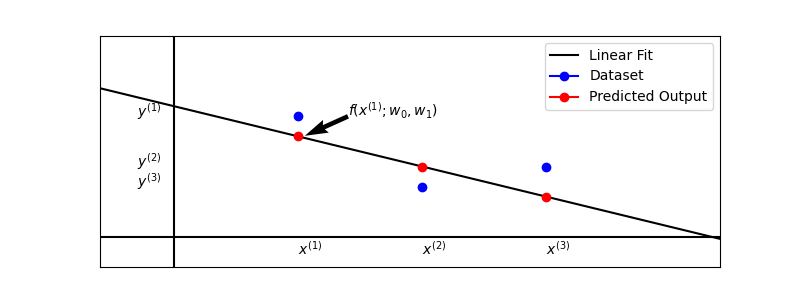
\includegraphics[scale=0.8]{lossfunction.png}
    \caption{Loss function and its Prediction}
\end{figure}
the fit is adjusted using the "squared loss" or the "residual squares" (RSS)
\begin{equation*}
    J(w_0, w_1) = \sum\limits_{n = 1}^{N}\left(y^{(n)} - f(x^{(n)};w_0;w_1)\right)^{2}
\end{equation*}

{\large\textbf{Optimization}}
Want to find $w_0,  w_1$ to minimise $J(w_0, w_1)$, $\hat{w_0}, \hat{w_1} = argmin_{w_0, w_1}J(w_0, w_1)$

strategy: Set $\frac{\partial J}{\partial w_0} = 0$ and $\frac{\partial J}{\partial w_1} = 0$
\[
    J(w_0, w_1) = \sum\limits_{n = 1}^{N}\left(y^{(n)} - f(x^{(n)};w_0, w_1)\right)^2 = \sum\limits_{n = 1}^{N}\left(y^{(n)} - (w_0 + w_1x^{(n)})\right)^2\\
\]
\begin{align*}
    \frac{\partial J}{\partial w_0} &= \sum\limits_{n = 1}^{N}\frac{\partial}{\partial w_0}\left(y^{(n)} - f(x^{(n)};w_0, w_1)\right)^2 = \sum\limits_{n = 1}^{N}2\left(y^{(n)} - w_0 - w_1x^{(n)}\right)(-1) = 0\\
    &\iff \sum\limits_{n = 1}^{N}w_0 = \sum\limits_{n = 1}^{N}y^{(n)} - w_1\sum\limits_{n = 1}^{N}x^{(n)} \iff Nw_0 = \sum\limits_{n = 1}^{N}y^{(n)} - w_1\sum\limits_{n = 1}^{N}x^{(n)}\\
    &\iff w_0 = \frac{1}{N}\sum\limits_{n = 1}^{N}y^{(n)} - w_1\frac{1}{N}\sum\limits_{n = 1}^{N}x^{(n)} \implies \hat{w_0} = \overline{y} - w_1\cdot\overline{x}
\end{align*}
Hat used to indicate particular value, bar used to indicate estimated mean, the same accours to $w_1$
\begin{align*}
    \frac{\partial J}{\partial w_1} &= \sum\limits_{n = 1}^{N}\frac{\partial}{\partial w_0}\left(y^{(n)} - f(x^{(n)};w_0, w_1)\right)^2 = \sum\limits_{n = 1}^{N}2\left(y^{(n)}-\overline{y} - w_1(x^{(n)}-\overline{x})\right)(-1)(x^{(n)}-\overline{x}) = 0\\
    &\implies \hat{w_1} = \frac{\sum\limits_{n  =1}^{N}(y^{(n)}-\overline{y})(x^{(n)} - \overline{x})}{\sum\limits_{n = 1}^{N}\left(x^{(n)}-\overline{x}\right)^2}
\end{align*}
These parameters settings are called the "least squared estimates".

For multiple linear regression, 
\begin{gather*}
    f(x_1, x_2, \dots, x_d; w_0, w_1, \dots, w_d) = w_0 + w_1x_1 + w_2x_2 + \dots + w_Dx_D = f(\mathbf{x}, \mathbf{w}) = \mathbf{w}^{T}\mathbf{x}\\
    \mathbf{w} = \left[
        \begin{array}{c}
        w_0\\
        w_1\\
        \vdots\\
        w_D
        \end{array}
        \right]\qquad and\qquad \mathbf{x} = \left[
            \begin{array}{c}
                1\\
                x_1\\
                \vdots\\
                x_D
            \end{array}
        \right]
\end{gather*}
{\Large\textbf{Loss function}}

Squared loss:
\begin{align*}
    J(\mathbf{w}) &= \sum\limits_{n = 1}^{N}(y^{(n)} - f(\mathbf{x}^{(n)};\mathbf{w}))^2\\
    &= \sum\limits_{n = 1}^{N}(y^{(n)} - (w_0 + w_1x_1^{(n)} + \dots + w_Dx_D^{(n)}))^2
\end{align*}

Derivating, $\frac{\partial J}{\partial w_0}, \frac{\partial J}{\partial w_1},\dots, \frac{\partial J}{\partial w_D}$ and set equal to zero, $\frac{\partial J}{\partial\mathbf{w}} = 0$, getting the followoing result
\begin{align*}
    \mathbf{\hat{w}} = (\mathbf{x}^{T}\mathbf{x})^{-1}\mathbf{x}^{T}\mathbf{y}
\end{align*}
This is called the normal equation.




\end{document}